\subsubsection{Sampling the Position of First Return}%
\label{sec:sampling_the_location_of_first_return}
Now that we have a ``\emph{mandatory boundary}'' $k$, we just need to sample a position $x$ with height $h = x_i-k+1$.
In fact, we will do something stronger by sampling the \emph{first} time the walk touches the boundary after $x_i$.
\begin{figure}[htpb]
    \centering
    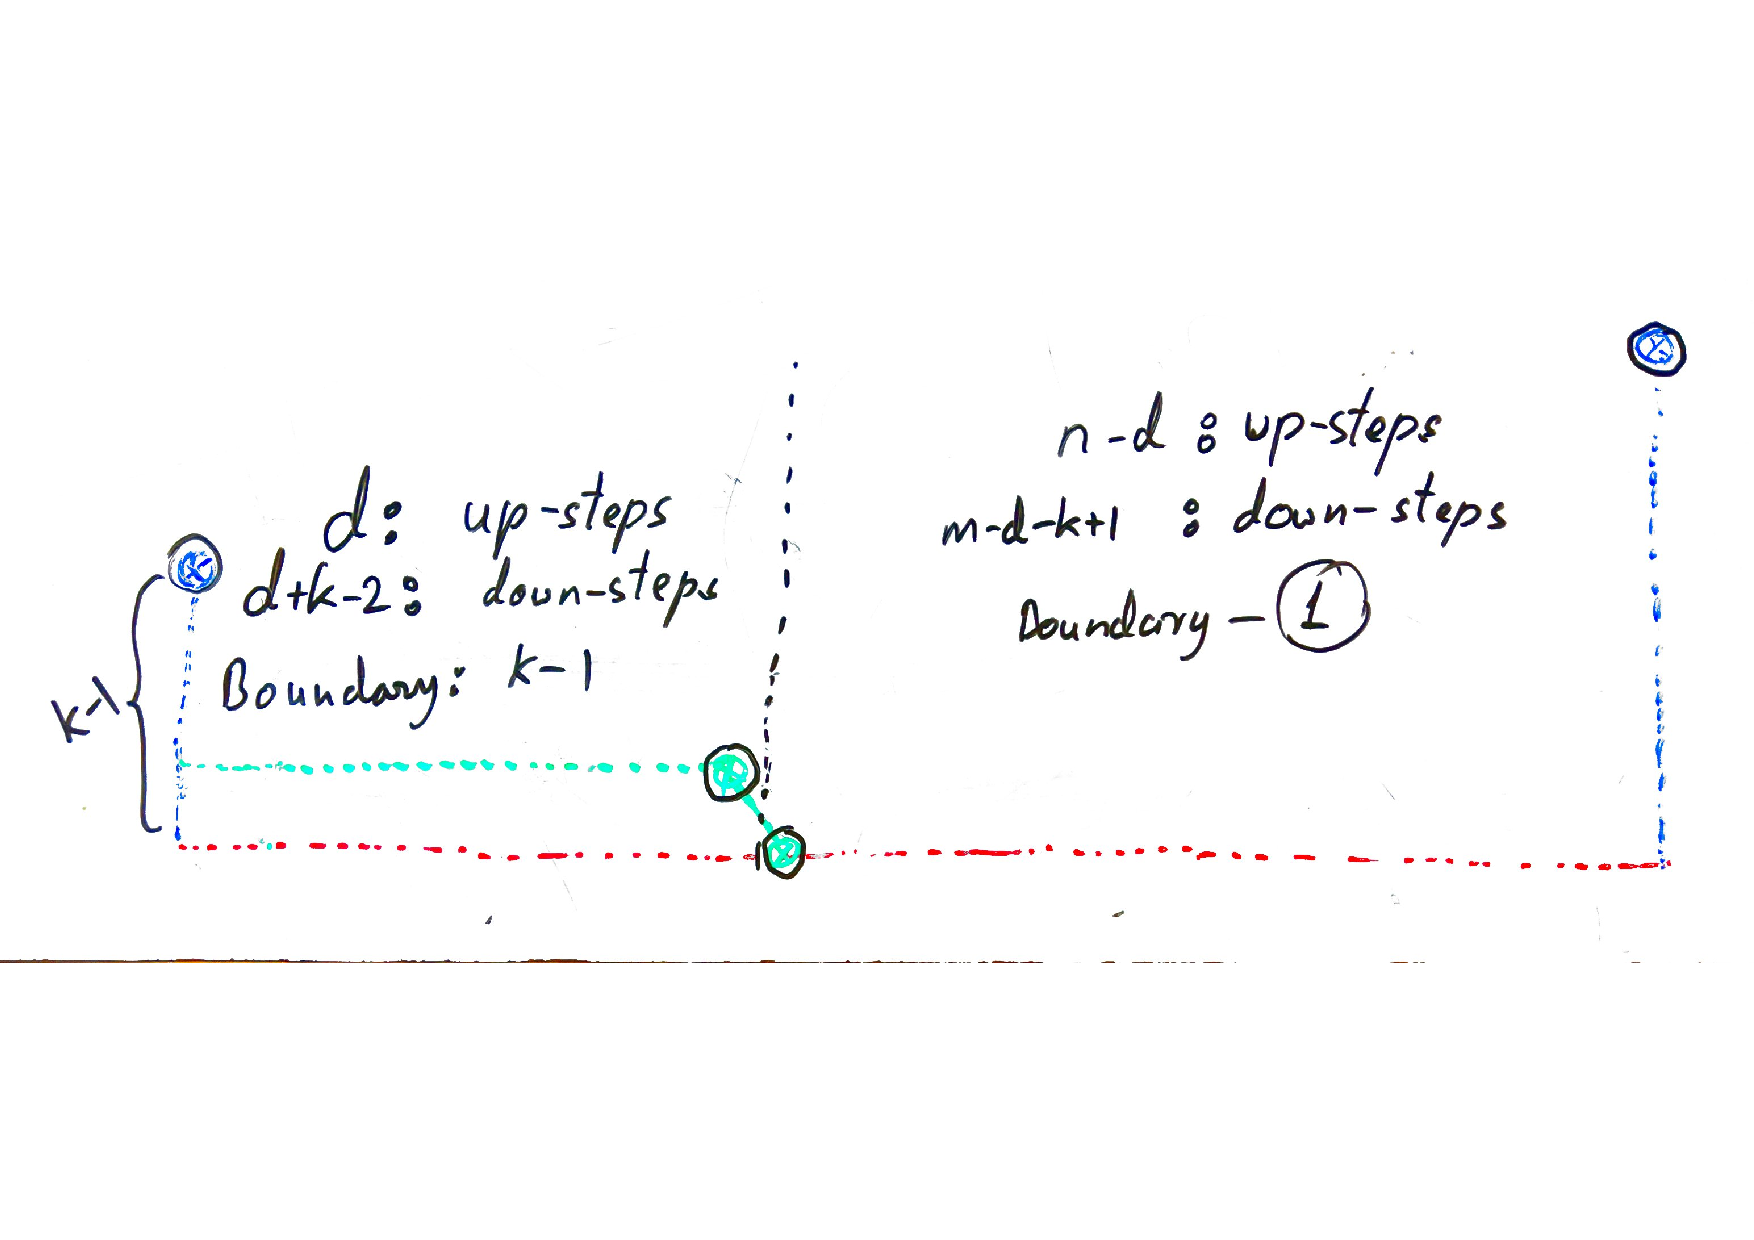
\includegraphics[width=1.0\linewidth, trim={0 6cm 0 5cm}]{images/dyck_return_sampling.pdf}
    \caption{Zooming into (and flipping) the error in Figure~\ref{fig:dyck_return_sampling}}
    \label{fig:dyck_return_sampling}
\end{figure}

We will parameterize the position $x$ the number of up-steps between $x_i$ and $x$
(See Figure~\ref{fig:dyck_return_sampling}).
This quantity will be referred to as $d$ such that $x - x_{i+1} = 2d + k-1$.
Given a specific $d$, we want to compute the number of valid paths that result in
$d$ up-steps before the first approach to the boundary.
We will calculate this quantity by counting the total number of paths to the left and right
of the first approach and multiplying them together.

Since we only care about getting a asymptotic (up to $\poly(\log n)$ factors) estimate of the probabilities,
it suffices to estimate the number of paths asymptotically as well.

\begin{restatable}{lemma}{ReturnDLeftBound}
\label{lem:ReturnDLeftBound}
If $d > \log^7 n$, then $D_{left}(d)
= \Theta\left( \frac{2^{2d+k}}{\sqrt{d}}\mathlarger e^{-r_{left}(d)}\cdot \frac{k-1}{d+k-1}\right)$
where $r_{left}(d) = \frac{(k-2)^2}{2(2d+k-2)}$.
\end{restatable}
\todo{Deal with smaller values of $d$}

\begin{restatable}{lemma}{ReturnDRightBound}
\label{lem:ReturnDRightBound}
If $U+D-2d-k > \log^7 n$, then $D_{right}(d)
= \Theta\left( \frac{2^{U+D-2d-k}}{\sqrt{U+d-2d-k}}\mathlarger e^{-r_{right}(d)}\cdot \frac{U-D+k}{U-d+1}\right)$
where $r_{right}(d) = \frac{(U-D-k-1)^2}{4(U+D-2d-k+1)}$.
\end{restatable}
\todo{Deal with other values of $d$}


\subsubsection{Estimating the CDF}%
\label{ssub:estimating_the_cdf}

\begin{restatable}{lemma}{ReturnProbabilityBoundNotNormalized}
\label{lem:ReturnProbabilityBoundNotNormalized}
$D_{left}(d)\cdot D_{right}(d)
= \Theta\left( \frac{2^{U+D}}{\sqrt{d(U+D-2d-k)}}\mathlarger e^{-r(d)}\cdot\frac{k-1}{d+k-1}\cdot\frac{U-D+k}{U-d+1}\right)$
where $r(d)=\mathcal O(\log^2 n)$.
\end{restatable}
\begin{proof}
This follows from the fact that both $r_{left}(d)$ and $r_{right}(d)$ are $\mathcal O(\log^2 n)$.
\end{proof}

\begin{corollary}
\label{cor:ReturnProbabilityRounding}
The probability $p_d$ of sampling $d$ as the number of up-steps
before the first approach to the boundary can be approximated as:
\[
p_d = \Theta\left( \frac{ 2^{U+D}\cdot\frac{(k-1)(U-D+k)}{\sqrt{d(U+D-2d-k)}(d+k-1)(U-d+1)}\cdot
\mathlarger e^{-\floor{r(d)}} }{\binom{U+D}{U}-\binom{U+D}{D-k}} \right)
\]
\todo{$D_{total}$ is not correct}
This is because the floor function only affects the value of the exponential by a factor of at most $e$.
\end{corollary}
\begin{corollary}
\label{cor:ReturnProbabilityPiecewiseContinuous}
We define a piecewise continuous function
\[
\hat q(d) = \frac{ 2^{U+D}\cdot\frac{(k-1)(U-D+k)}{\sqrt{d(U+D-2d-k)}(d+k-1)(U-d+1)}\cdot
\mathlarger e^{-\floor{r(d)}} }{\binom{U+D}{U}-\binom{U+D}{D-k}}
\]
We claim that $p_d = \Theta\left( \int\limits_d^{d+1} \hat q(d)\right)$.
Note that this integral has a closed form for a fixed value of $\floor{r(d)}$.
\end{corollary}


Let the maximum value of $r(d)$ be $r_{max} = \mathcal O(\log^2 n)$.
\begin{corollary}
\label{cor:}
We can compute the approximate normalized probabilities
\[
q_d = \frac{\int\limits_d^{d+1} \hat q(d)}{\int\limits_1^{n} \hat q(d)}
\]
such that $p_d = \Theta(q_d)$.
Furthermore, we can also compute the CDF of $q_d$ as:
\[
Q_d = \frac{\int\limits_1^{d+1} \hat q(d)}{\int\limits_1^{n} \hat q(d)}
\]
This allows us to sample from the distribution $q_d$ and use Lemma~\ref{lem:huge} to indirectly sample from $p_d$.
\end{corollary}

